% Innehållet i Vasungavisor 2018
%
% Kapitel "Blomdoft I Melodin"

\songchapter{Blomdoft I Melodin}
\chapterimage[width=0.8\textwidth]{../bilder/fardigabilder/BilderTillKapitel/lalala.png} 

% Exempel på färdig-formaterad sång till VN:s
% sångbok 2018.

% Denna fil kan användas som sådan, bara verserna,
% namnen och annan rådata behöver bytas ur fälten.
% Tecknet "%" markerar en kommentar som helt och 
% hållet ignoreras av programmet som läser filen.

% Spara den färdiga filen som 
% 'SangnamnUtanMellanslagEllerSkander.tex'
% t.ex. blir "Vid En Källa" till 
% 'VidEnKalla.tex'
% Varje sång blir en egen fil.

\beginsong{Balladen om Fredrik Åkare}[ 	% Börja sången här
	by={Cornelis Vreeswijk},	% Författare
	sr={Monday morning}]		% Alternativa
			% sångnamn
	
\beginverse*		% Börja vers
Från Öckerö loge hörs dragspel och bas
och fullmånen lyser som var den av glas.
Där dansar Fredrik Åkare kind emot kind
med lilla fröken Cecilia Lind.
\endverse			% Sluta vers

\beginverse*		% Börja vers
Hon dansar och blundar så nära intill,
hon följer i dansen precis vart han vill.
Han för och hon följer så lätt som en vind,
Men säg varför rodnar Cecilia Lind?
\endverse			% Sluta vers

\beginverse*		% Börja vers
Säg var det för det Fredrik Åkare sa:
Du doftar så gott och du dansar så bra.
Din midja är smal och barmen är trind.
Vad du är vacker, Cecilia Lind.
\endverse			% Sluta vers

\beginverse*		% Börja vers
Men dansen tog slut och vart skulle dom gå?
Dom bodde så nära varandra ändå.
Till slut kom dom fram till Cecilias grind.
Nu vill jag bli kysst, sa Cecilia Lind.
\endverse			% Sluta vers

\beginverse*		% Börja vers
Vet hut, Fredrik Åkare, skäms gamla karln!
Cecilia Lind är ju bara ett barn.
Ren som en blomma, skygg som en hind.
Jag fyller snart sjutton, sa Cecilia Lind.
\endverse			% Sluta vers

\beginverse*		% Börja vers
Och stjärnorna vandra och timmarna fly
och Fredrik är gammal men månen är ny.
Ja, Fredrik är gammal men kärlek är blind.
Åh, kyss mig igen, sa Cecilia Lind.
\endverse			% Sluta vers
\endsong			% Sluta sång

\sclearpage
% Exempel på färdig-formaterad sång till VN:s
% sångbok 2018.

% Denna fil kan användas som sådan, bara verserna,
% namnen och annan rådata behöver bytas ur fälten.
% Tecknet "%" markerar en kommentar som helt och 
% hållet ignoreras av programmet som läser filen.

% Spara den färdiga filen som 
% 'SangnamnUtanMellanslagEllerSkander.tex'
% t.ex. blir "Vid En Källa" till 
% 'VidEnKalla.tex'
% Varje sång blir en egen fil.

\beginsong{Calle Schewens vals}[ 	% Börja sången här
	by={Evert Taube},	% Författare
	sr={},
	index={I Roslagens famn}]		% Melodi
			% Alternativa
			% sångnamn
	
\beginverse*		% Börja vers
I Roslagens famn på den blommande ö,
där vågorna klucka mot strand
och vassarna vagga och nyslaget hö
det doftar emot oss ibland,
där sitter jag uti bersån på en bänk
och tittar på tärnor och mås,
som störta mot fjärden i glitter och stänk
på jakt efter födan, gunås.
\endverse			% Sluta vers

\beginverse*		% Börja vers
Själv blandar jag fredligt mitt kaffe med kron
till angenäm styrka och smak
och lyssnar till dragspelets lockande ton,
som hörs från mitt stugogemak.
Jag är som en pojke, fast farfar jag är,
ja rospiggen spritter i mig!
Det blir bara värre med åren det där
med dans och med jäntornas blig.
\endverse			% Sluta vers

\beginverse*		% Börja vers
Se, måsen med löjan i näbb, han fick sitt!
Men jag fick en arm om min hals!
O, eviga ungdom, mitt hjärta är ditt,
spel opp, jag vill dansa en vals.
Det doftar, det sjunger från skog och från sjö,
i natt ska du vara min gäst!
Här dansar Calle Schewen med Roslagens mö
och solen går ned i nordväst.
\endverse			% Sluta vers

\beginverse*		% Börja vers
Då vilar min blommande ö vid min barm,
du dunkelblå, vindstilla fjärd
och juninattsskymningen smyger sig varm
till sovande buskar och träd.
Min älva, du dansar så lyssnande tyst
och tänker, att karlar är troll.
Den skälver, din barnsliga hand, som jag kysst,
och valsen förklingar i moll.
\endverse			% Sluta vers

\beginverse*		% Börja vers
Men hej, alla vänner, som gästa min ö!
Jag är både nykter och klok!
När morgonen gryr, ska jag vålma mitt hö
och vittja tvåhundrade krok.
Fördöme dig skymning, och drag nu din kos!
Det brinner i martallens topp!
Här dansar Calle Schewen med Roslagens ros
han dansar till solen går opp!
\endverse			% Sluta vers
\textnote{Sången sponsoreras av Vasa nations styrelseordföranden 2003 och 2006 Marie och Martin Sjölind.}
\endsong			% Sluta sång

\begin{intersong}
\begin{center}
\includegraphics[width=15mm]{../bilder/varsomhelst.jpg} 
\end{center}
\end{intersong}
\sclearpage
% Exempel på färdig-formaterad sång till VN:s
% sångbok 2018.

% Denna fil kan användas som sådan, bara verserna,
% namnen och annan rådata behöver bytas ur fälten.
% Tecknet "%" markerar en kommentar som helt och 
% hållet ignoreras av programmet som läser filen.

% Spara den färdiga filen som 
% 'SangnamnUtanMellanslagEllerSkander.tex'
% t.ex. blir "Vid En Källa" till 
% 'VidEnKalla.tex'
% Varje sång blir en egen fil.

\beginsong{En sjöman älskar havets våg}[ 	% Börja sången här
	by={Gustaf Arthur Ossian Limborg},	% Författare
	sr={},		% Melodi
	index={Ålandsvisan}]		% Alternativa
			% sångnamn
	
\beginverse*		% Börja vers
En sjöman älskar havets våg, 
ja vågornas brus.
När stormen skakar mast och tåg, 
hör stormarnas sus!
\endverse			% Sluta vers

\beginchorus
:,: Farväl, farväl förtjusande mö! 
Vi komma väl snart igen. :,:
\endchorus

\beginverse*		% Börja vers
Hon trycker då så ömt min hand 
vid vågornas brus.
Då känns det tungt att gå från land 
till stormarnas sus.
\endverse			% Sluta vers

\beginchorus
:,: Farväl, farväl... :,:
\endchorus

\beginverse*		% Börja vers
Hon viskar ömt och ljuvt mitt namn 
vid vågornas brus.
Kom snart tillbaka i min famn 
från stormarnas sus.
\endverse			% Sluta vers

\beginchorus
:,: Farväl, farväl... :,:
\endchorus

\beginverse*		% Börja vers
Min trogna flickas varma kyss 
hör vågornas brus 
för sista gången fick jag nyss. 
Hör stormarnas sus!
\endverse			% Sluta vers

\beginchorus
:,: Farväl, farväl... :,:
\endchorus
\endsong			% Sluta sång

\sclearpage
% Exempel på färdig-formaterad sång till VN:s
% sångbok 2018.

% Denna fil kan användas som sådan, bara verserna,
% namnen och annan rådata behöver bytas ur fälten.
% Tecknet "%" markerar en kommentar som helt och 
% hållet ignoreras av programmet som läser filen.

% Spara den färdiga filen som 
% 'SangnamnUtanMellanslagEllerSkander.tex'
% t.ex. blir "Vid En Källa" till 
% 'VidEnKalla.tex'
% Varje sång blir en egen fil.

\beginsong{Där björkarna susa}[ 	% Börja sången här
	by={Viktor Sund}]		% Melodi
			% Alternativa
			% sångnamn
	
\beginverse*		% Börja vers
Där björkarna susa sin milda sommarsång
och ängen av rosor blommar,
skall vårt strålande brudefölje en gång
draga fram i den ljuvliga sommar.
\endverse			% Sluta vers

\beginverse*		% Börja vers
Där barndomstidens minne sväva ljust omkring
och drömmarna på barndomsstigar vandra,
där skola vi i sommar växla tro och ring
och lova att älska varandra.
\endverse			% Sluta vers

\beginverse*		% Börja vers
Där björkarna susa, där skola vi bland dem
svära trohet och kärlek åt varandra.
Där skola vi se'n bygga vår unga lyckas hem
och göra livet ljuvligt för varandra.
\endverse			% Sluta vers
\endsong			% Sluta sång

\begin{intersong}
\begin{center}
\includegraphics[width=4cm]{../bilder/eloveena.jpg} 
\end{center}
\end{intersong}
\sclearpage
% Exempel på färdig-formaterad sång till VN:s
% sångbok 2018.

% Denna fil kan användas som sådan, bara verserna,
% namnen och annan rådata behöver bytas ur fälten.
% Tecknet "%" markerar en kommentar som helt och 
% hållet ignoreras av programmet som läser filen.

% Spara den färdiga filen som 
% 'SangnamnUtanMellanslagEllerSkander.tex'
% t.ex. blir "Vid En Källa" till 
% 'VidEnKalla.tex'
% Varje sång blir en egen fil.

\beginsong{Fredmans epistel nr 64}[ 	% Börja sången här
	by={Carl Michael Bellman}, % Författare	% Melodi
	index={Fjäriln vingad syns på Haga}]	% Alternativa
			% sångnamn
	
\beginverse*		% Börja vers
Fjäriln vingad syns på Haga
mellan dimmors frost och dun.
Sig sitt gröna skjul tillaga
och blomman i sin paulun;
minsta kräk i kärr och syra,
nyss av solens värma väckt,
till en ny högtidlig yra
eldas vid sefirens fläkt.
\endverse			% Sluta vers

\beginverse*		% Börja vers
Haga, i ditt sköte röjes
gräsets brodd och gula plan;
stolt i dina rännlar höjes
gungande den vita svan.
Längst ur skogens glesa kamrar
höras täta återskall,
än från den graniten hamrar,
än från yx i björk och tall.
\endverse			% Sluta vers
\endsong			% Sluta sång

\begin{intersong}
\begin{center}
\includegraphics[width=17mm]{../bilder/fjaril.jpg} 
\end{center}
\end{intersong}
\sclearpage
% Exempel på färdig-formaterad sång till VN:s
% sångbok 2018.

% Denna fil kan användas som sådan, bara verserna,
% namnen och annan rådata behöver bytas ur fälten.
% Tecknet "%" markerar en kommentar som helt och 
% hållet ignoreras av programmet som läser filen.

% Spara den färdiga filen som 
% 'SangnamnUtanMellanslagEllerSkander.tex'
% t.ex. blir "Vid En Källa" till 
% 'VidEnKalla.tex'
% Varje sång blir en egen fil.

\beginsong{Har du visor min vän}[ 	% Börja sången här
	by={Bengt Ahlfors}]		% Alternativa
			% sångnamn
	
\beginverse*		% Börja vers
Har du visor min vän, sjung dem nu!
För nu är tiden då visor ska sjungas
och den som ska sjunga är du!
I morgon är kanske för sent, min vän.
Så synd om de sånger som aldrig blir sjungna!
Så tala inte om visor med mig.
Låt visorna tala för dig. 
\endverse			% Sluta vers

\beginverse*		% Börja vers
Vill du älska min vän, gör det nu!
För nu är tiden för kärlek inne
och den som ska älska är du!
I morgon är kanske för sent, min vän.
Så synd om den längtan som aldrig har vågat!
Så tala inte om kärleken.
Låt kärleken tala min vän. 
\endverse			% Sluta vers

\beginverse*		% Börja vers
Vill du leva ditt liv, gör det nu!
För nu är tiden då ditt liv ska levas
och den som ska leva är du!
I morgon är kanske för sent, min vän.
Vem bryr sig då om vad du drömde och ville?
Så vänta inte på någonting sen.
Det är nu du ska leva min vän! 
\endverse			% Sluta vers

\textnote{Sången sponsoreras av Vasa nations inspektor 1997-2005 Mathias ``Matti'' Klockars.}

\endsong			% Sluta sång

\sclearpage
% Exempel på färdig-formaterad sång till VN:s
% sångbok 2018.

% Denna fil kan användas som sådan, bara verserna,
% namnen och annan rådata behöver bytas ur fälten.
% Tecknet "%" markerar en kommentar som helt och 
% hållet ignoreras av programmet som läser filen.

% Spara den färdiga filen som 
% 'SangnamnUtanMellanslagEllerSkander.tex'
% t.ex. blir "Vid En Källa" till 
% 'VidEnKalla.tex'
% Varje sång blir en egen fil.

\beginsong{Höstvisa}[ 	% Börja sången här
	by={Tove Jansson},
	index={Skynda dig älskade},
	index={Vägen hem var mycket lång}]		% Alternativa
			% sångnamn
	
\beginverse*		% Börja vers
Vägen hem var mycket lång och ingen har jag mött,
nu blir kvällarna kyliga och sena.
Kom trösta mig en smula, för nu är jag ganska trött,
och med ens så förfärligt allena.
Jag märkte aldrig förut, att mörkret är så stort,
går och tänker på allt det där man borde.
Det finns så mycket saker jag skulle sagt och gjort,
och det är så väldigt lite jag gjorde.
\endverse			% Sluta vers

\beginchorus
Skynda dig älskade, skynda att älska,
dagarna mörkna minut för minut.
Tänd våra ljus, det är nära till natten,
snart är den blommande sommarn slut.
\endchorus

\beginverse*		% Börja vers
Jag letar efter nånting som vi kanske glömde bort
och som du kunde hjälpa mig att finna.
En sommar går förbi, den är alltid lika kort,
den är drömmen om det man kunnat vinna.
Du kommer kanske nångång, förr'n skymningen blir blå
innan ängarna blir torra och tomma.
Kanske hittar vi varann, kanske hittar vi då på
något sätt att få allting att blomma.
\endverse			% Sluta vers

\beginchorus
Skynda dig älskade, skynda att älska...
\endchorus

\newpage
\beginverse*		% Börja vers
Nu blåser storm därute och stänger sommarns dörr,
det är för sent för att undra och leta.
Jag älskar kanske mindre än vad jag gjorde förr
men mer än du nånsin får veta.
Nu ser vi alla fyrar kring höstens långa kust
och hör vågorna villsamma vandra.
En enda sak är viktig och det är hjärtats lust
och att få vara samman med varandra.
\endverse			% Sluta vers

\beginchorus
Skynda dig älskade, skynda att älska...
\endchorus
\endsong			% Sluta sång

\sclearpage
% Exempel på färdig-formaterad sång till VN:s
% sångbok 2018.

% Denna fil kan användas som sådan, bara verserna,
% namnen och annan rådata behöver bytas ur fälten.
% Tecknet "%" markerar en kommentar som helt och 
% hållet ignoreras av programmet som läser filen.

% Spara den färdiga filen som 
% 'SangnamnUtanMellanslagEllerSkander.tex'
% t.ex. blir "Vid En Källa" till 
% 'VidEnKalla.tex'
% Varje sång blir en egen fil.

\beginsong{Jag tror på sommaren}[ 	% Börja sången här
	by={Stig Olin}]		% Melodi
			% Alternativa
			% sångnamn

\beginverse*		% Börja vers
Kortast och blekast vintersol
finns en decemberdag
kallad för Thomas Tvivlaren
för att hans tro var svag.
Man skulle aldrig någonsin
trott på en sol, en vår.
Ändå förvandlas vintern till 
sommar vartenda år.
\endverse			% Sluta vers

\beginchorus
Jag tror, jag tror på sommaren.
Jag tror, jag tror på sol igen.
Jag pyntar mig i blå kravatt
och hälsar dig med blommig hatt.
Jag tror på dröm om sommarhus
med täppa och med lindars sus.
En speleman med sin fiol
och luften fylld av kaprifol.
\endchorus

\beginverse*		% Börja vers
Midsommarafton, natten lång
kärlek och dans och sång.
Solen som plötsligt börjar gå
upp och ner på samma gång.
Pojken med flickans hand i sin
viskar och får till svar
löften han gått och hoppats på 
under det år som var.
\endverse			% Sluta vers

\beginchorus
Jag tror, jag tror …
\endchorus
\endsong			% Sluta sång

\sclearpage
% Exempel på färdig-formaterad sång till VN:s
% sångbok 2018.

% Denna fil kan användas som sådan, bara verserna,
% namnen och annan rådata behöver bytas ur fälten.
% Tecknet "%" markerar en kommentar som helt och 
% hållet ignoreras av programmet som läser filen.

% Spara den färdiga filen som 
% 'SangnamnUtanMellanslagEllerSkander.tex'
% t.ex. blir "Vid En Källa" till 
% 'VidEnKalla.tex'
% Varje sång blir en egen fil.

\beginsong{Men liljorna de växa upp om våren}[ 	% Börja sången här
	by={Alexander Slotte},	% Författare			% Melodi
	index={De gamlas hälsning till brudparet}]		% Alternativa
			% sångnamn
	
\beginverse*		% Börja vers
Och glädjen den dansar bland blommor och strå.
Men åren de komma och åren de gå.
Då blir det så stilla kring vännerna två.
Men liljorna de växa upp om våren.
\endverse			% Sluta vers

\beginverse*		% Börja vers
Och världen är så vider och världen är så stor
och sorgerna, de komma från sunnan och från nord.
Då är det gott i stugan, där kärleken bor.
Och liljorna de växa upp om våren.
\endverse			% Sluta vers

\beginverse*		% Börja vers
Och människorna födas och människorna dö,
som gångande vågor på villande sjö.
De fallande blomstren ska' täckas av snö.
Men liljorna de växa upp om våren.
\endverse			% Sluta vers
\endsong			% Sluta sång

\sclearpage
% Exempel på färdig-formaterad sång till VN:s
% sångbok 2018.

% Denna fil kan användas som sådan, bara verserna,
% namnen och annan rådata behöver bytas ur fälten.
% Tecknet "%" markerar en kommentar som helt och 
% hållet ignoreras av programmet som läser filen.

% Spara den färdiga filen som 
% 'SangnamnUtanMellanslagEllerSkander.tex'
% t.ex. blir "Vid En Källa" till 
% 'VidEnKalla.tex'
% Varje sång blir en egen fil.

\beginsong{Plocka vill jag skogsviol}[ 	% Börja sången här
	by={Alexander Slotte}]		% Alternativa
			% sångnamn
	
\beginverse*		% Börja vers
Plocka vill jag skogsviol och 
ljungens fina frans, 
plocka, plocka famnen full och 
binda till en krans. 
Vintergrön och timje 
minna mig om vännen min, och 
många, många tankar jag i 
kransen binder in. 
\endverse			% Sluta vers

\beginverse*		% Börja vers
Här är stigen, som vi gått i 
söndagsstilla kväll. 
Här vi suttit hand i hand på 
mossbelupen häll. 
Är det ock en annan, 
som du givit har din hand, 
jag blir dig huld, du är dock min i 
mina drömmars land. 
\endverse			% Sluta vers

\beginverse*		% Börja vers
Ensam är jag vorden här, och 
ensam skall jag gå. 
Ringa jag på jorden är och 
fattig likaså. 
Ingen kan dock taga 
från mig minnets lyckoskatt. Jag 
är så rik allt med min krans i 
sommarljuvlig natt. 
\endverse			% Sluta vers

\beginverse*		% Börja vers
Plocka vill jag skogsviol och 
ljungens fina frans, 
plocka, plocka famnen full och 
binda till en krans. 
Vintergrön och timje 
minna mig om vännen min, och 
många, många tankar jag i 
kransen binder in. 
\endverse			% Sluta vers
\endsong			% Sluta sång

\begin{intersong}
\begin{center}
	\vspace{20mm}
\includegraphics[width=4cm]{../bilder/ros.jpg} 
\end{center}
\end{intersong}
\sclearpage
% Exempel på färdig-formaterad sång till VN:s
% sångbok 2018.

% Denna fil kan användas som sådan, bara verserna,
% namnen och annan rådata behöver bytas ur fälten.
% Tecknet "%" markerar en kommentar som helt och 
% hållet ignoreras av programmet som läser filen.

% Spara den färdiga filen som 
% 'SangnamnUtanMellanslagEllerSkander.tex'
% t.ex. blir "Vid En Källa" till 
% 'VidEnKalla.tex'
% Varje sång blir en egen fil.

\beginsong{Så länge skutan kan gå}[ 	% Börja sången här
	by={Evert Taube}]		% Melodi
			% Alternativa
			% sångnamn
	
\beginverse*		% Börja vers
Så länge skutan kan gå,
så länge hjärtat kan slå,
så länge solen den glittrar på böljorna blå.
Om blott en dag eller två,
så håll till godo ändå,
för det finns många som aldrig en ljusglimt kan få.
\endverse			% Sluta vers

\beginverse*		% Börja vers
Och vem har sagt att just du kom till världen
för att få solsken och lycka på färden?
Att under stjärnornas glans
bli purrad ut i en skans,
att få en kyss eller två i en yrande dans?
Ja, vem har sagt att just du skall ha hörsel och syn,
höra böljornas brus och kunna sjunga?
Och vem har sagt att just du skall ha bästa menyn
och som fågeln på böljorna gunga?
\endverse			% Sluta vers

\beginverse*		% Börja vers
Och vid motorernas gång
och ifall vakten blir lång.
så minns att snart klämtar klockan för dig:
ding, ding, dång!
Så länge skutan kan gå,
så länge hjärtat kan slå,
så länge solen den glittrar på böljorna blå.
\endverse			% Sluta vers

\beginverse*		% Börja vers
Så tag med glädje ditt jobb fast du lider,
snart får du vila för eviga tider.
Men inget hindrar dig alls
att du är glad och ger hals,
så kläm i nu med en verkligt sjusjungande vals!
\endverse			% Sluta vers

\beginverse*		% Börja vers
Det är rasande tur att du lever, min vän,
och kan valsa omkring uti Havanna!
Om pengarna tagit slut gå till sjöss om igen 
med Karibiens passadvind kring pannan.
\endverse			% Sluta vers

\beginverse*		% Börja vers
Klara jobbet med glans,
gå iland någonstans,
ta en kyss eller två i en yrande dans!
Så länge skutan kan gå,
så länge hjärtat kan slå,
så länge solen den glittrar på böljorna blå.
\endverse			% Sluta vers
\endsong			% Sluta sång

\begin{intersong}
\begin{center}
	\vspace{20mm}
\includegraphics[width=0.8\textwidth]{../bilder/skargard.jpg} 
\end{center}
\end{intersong}
\sclearpage
% Exempel på färdig-formaterad sång till VN:s
% sångbok 2018.

% Denna fil kan användas som sådan, bara verserna,
% namnen och annan rådata behöver bytas ur fälten.
% Tecknet "%" markerar en kommentar som helt och 
% hållet ignoreras av programmet som läser filen.

% Spara den färdiga filen som 
% 'SangnamnUtanMellanslagEllerSkander.tex'
% t.ex. blir "Vid En Källa" till 
% 'VidEnKalla.tex'
% Varje sång blir en egen fil.

\beginsong{Sjösala vals}[ 	% Börja sången här
	by={Evert Taube},
	index={Rönnerdahl han skuttar}]		% Melodi
			% Alternativa
			% sångnamn
	
\beginverse*		% Börja vers
Rönnerdahl han skuttar med ett skratt ur sin säng
solen står på Orrberget, sunnanvind brusar.
Rönnerdahl han valsar över Sjösala äng.
Hör min vackra visa, kom sjung min refräng!
Tärnan har fått ungar och dyker i min vik,
ur alla gröna dungar hörs finkarnas musik.
Och se, så många blommor
som redan slagit ut på ängen!
Gullviva, mandelblom, kattfot och blå viol.
\endverse			% Sluta vers

\beginverse*		% Börja vers
Rönnerdahl han virvlar sina lurviga ben
under vita skjortan som viftar kring vaderna.
Lycklig som en lärka uti majsolen sken,
sjunger han för ekorrn som gungar på gren!
Kurre, kurre, kurre, nu dansar Rönnerdahl
Koko! Och göken ropar uti hans gröna dal.
Och se, så många blommor
som redan slagit ut på ängen!
Gullviva, mandelblom, kattfot och blå viol.
\endverse			% Sluta vers

\newpage
\beginverse*		% Börja vers
Rönnerdahl han binder utav blommor en krans,
binder den kring håret, det gråa och rufsiga,
valsar in i stugan och har lutan till hands,
väcker frun och barnen med drill och kadans.
``Titta!'' ropar ungarna, ``Pappa är en brud 
med blomsterkrans i håret och nattskjortan till skrud!
Och se, så många blommor 
som redan slagit ut på ängen!
Gullviva, mandelblom, kattfot och blå viol.''
\endverse			% Sluta vers

\beginverse*		% Börja vers
Rönnerdahl är gammal, men han valsar ändå,
Rönnerdahl har sorger och ont om sekiner.
Sällan får han rasta – han får slita för två.
Hur han klarar skivan kan ingen förstå.
Ingen, utom tärnan i viken – hon som dök
och ekorren och finken och vårens första gök.
Och blommorna, de blommor
som redan slagit ut på ängen,
gullviva, mandelblom, kattfot och blå viol.
\endverse			% Sluta vers
\endsong			% Sluta sång

\sclearpage
% Exempel på färdig-formaterad sång till VN:s
% sångbok 2018.

% Denna fil kan användas som sådan, bara verserna,
% namnen och annan rådata behöver bytas ur fälten.
% Tecknet "%" markerar en kommentar som helt och 
% hållet ignoreras av programmet som läser filen.

% Spara den färdiga filen som 
% 'SangnamnUtanMellanslagEllerSkander.tex'
% t.ex. blir "Vid En Källa" till 
% 'VidEnKalla.tex'
% Varje sång blir en egen fil.

\beginsong{Svinnsta skär}[ 	% Börja sången här
	by={Gideon Wahlberg},
	index={Dansen den går uppå }]		% Melodi
			% Alternativa
			% sångnamn
	
\beginverse*		% Börja vers
Dansen den går uppå Svinnsta skär
hör klackarna mot hällen.
Gossen han svänger med flickan kär
i stilla sommarnatt.
Blommorna doftar från hagen där
och många andra ställen,
och mitt i taltrastens kvällskonsert
hörs många muntra skratt.
\endverse			% Sluta vers

\beginchorus	
Ljuvlig är sommarnatten
blånande vikens vatten
och mellan bergen och tallarna
höres musiken och trallarna.
Flickan har blommor i håret,
månen strör silver i snåret.
Aldrig förglömmer jag stunderna där
uppå Svinnsta skär.
\endchorus

\beginverse*		% Börja vers
Gossen tar flickan uti sin hand 
och vandrar neråt stranden,
lossar sin julle och ror från land, 
bland klippor och bland skär.
Drömmande ser han mot vågens rand
som rullar in mot stranden.
Kysser sin flicka så ömt ibland, 
och viskar ''Hjärtans kär''.
\endverse			% Sluta vers

\beginchorus	
Ljuvlig är sommarnatten...
\endchorus

\beginverse*		% Börja vers
Solen går upp bakom Konungssund, 
och stänker guld på vågen,
Fåglarna kvittra i varje lund, 
sin stilla morgonbön.
Gäddorna slå invid skär och grund, 
så lekfulla i hågen.
Men sista valsen i morgonstund, 
man hör från Svinnerön.
\endverse			% Sluta vers

\beginchorus	
Ljuvlig är sommarnatten...
\endchorus
\endsong			% Sluta sång

\begin{intersong}
	\begin{center}
		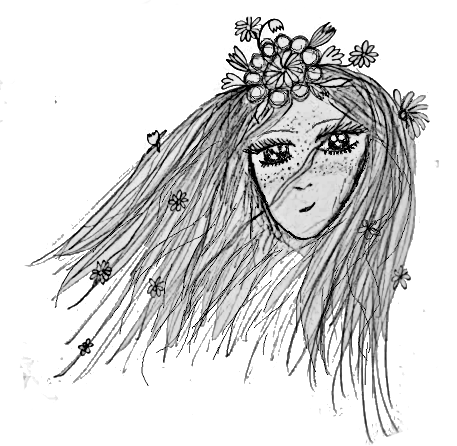
\includegraphics[width=0.7\textwidth]{../bilder/fardigabilder/CamillasFardigaBilder/Svinstaskar2.png} 
	\end{center}
\end{intersong}
\sclearpage
% Exempel på färdig-formaterad sång till VN:s
% sångbok 2018.

% Denna fil kan användas som sådan, bara verserna,
% namnen och annan rådata behöver bytas ur fälten.
% Tecknet "%" markerar en kommentar som helt och 
% hållet ignoreras av programmet som läser filen.

% Spara den färdiga filen som 
% 'SangnamnUtanMellanslagEllerSkander.tex'
% t.ex. blir "Vid En Källa" till 
% 'VidEnKalla.tex'
% Varje sång blir en egen fil.

\beginsong{Vårvindar friska}[ 	% Börja sången här
	by={Julia Nyberg}]		% Melodi
			% Alternativa
			% sångnamn
	
\beginverse*		% Börja vers
Vårvindar friska, leka och viska
lunderna kring, likt älskande par.
Strömmarna ila, finna ej vila,
förrän i havet störtvågen far.
Klappa mitt hjärta, klaga och hör.
Valthornets klang kring klipporna dör.
Strömkarlen spelar, sorgerna delar
vakan kring berg och dal.
\endverse			% Sluta vers
\endsong			% Sluta sång

\begin{intersong}
	\begin{center}
		\vspace{20mm}
		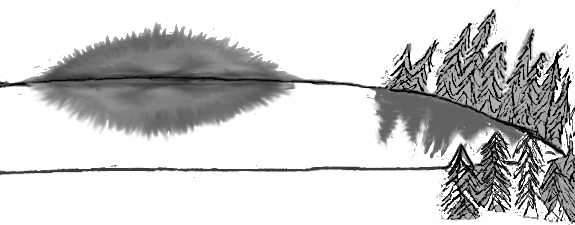
\includegraphics[width=1\textwidth]{../bilder/fardigabilder/CamillasFardigaBilder/Oppnalandskap3.png} 
	\end{center}
\end{intersong}
\sclearpage
% Exempel på färdig-formaterad sång till VN:s
% sångbok 2018.

% Denna fil kan användas som sådan, bara verserna,
% namnen och annan rådata behöver bytas ur fälten.
% Tecknet "%" markerar en kommentar som helt och 
% hållet ignoreras av programmet som läser filen.

% Spara den färdiga filen som 
% 'SangnamnUtanMellanslagEllerSkander.tex'
% t.ex. blir "Vid En Källa" till 
% 'VidEnKalla.tex'
% Varje sång blir en egen fil.

\beginsong{Visa vid vindens ängar}[ 	% Börja sången här
	by={Mats Paulson},
	index={Det går en vind}]		% Alternativa
			% sångnamn
	
\beginverse*		% Börja vers
Det går en vind över vindens ängar,
det fladdrar till i en tyllgardin.
Och jag ska skriva en sommarvisa
med sol och blomdoft i melodin.
Jag ville sjunga om Katarina,
till träklangsflöjter och alcymbal
men vindens toner blir sommarns sånger,
jag bara lyssnar i björklövssal.
Det går en vind över vindens ängar,
det fladdrar till i en tyllgardin.
Och jag ska skriva en sommarvisa
med sol och blomdoft i melodin.
\endverse			% Sluta vers

\beginverse*		% Börja vers
Det går en flicka i aspelunden,
jag har ett gulnat fotografi.
Med åren blev hon en dröm, en saga,
en ensam vandrares sympati.
Jag ville skriva en liten visa
där ögonblick blir till evighet
men ord blir stumma och toner döda
och visans tanke blir hemlighet.
Det går en flicka i aspelunden,
jag har ett gulnat fotografi.
Med åren blev hon en dröm, en saga,
en ensam vandrares sympati.
\endverse			% Sluta vers
\endsong			% Sluta sång

\begin{intersong}
\begin{center}
\includegraphics[scale=.4]{../bilder/tyllgardin.jpg} 
\end{center}
\end{intersong}

\sclearpage

% Exempel på färdig-formaterad sång till VN:s
% sångbok 2018.

% Denna fil kan användas som sådan, bara verserna,
% namnen och annan rådata behöver bytas ur fälten.
% Tecknet "%" markerar en kommentar som helt och 
% hållet ignoreras av programmet som läser filen.

% Spara den färdiga filen som 
% 'SangnamnUtanMellanslagEllerSkander.tex'
% t.ex. blir "Vid En Källa" till 
% 'VidEnKalla.tex'
% Varje sång blir en egen fil.

\beginsong{Mälarö Kyrka}[ 	% Börja sången här
	by={Sven Lindahl}]		% Melodi
			% Alternativa
			% sångnamn

\beginverse*		% Börja vers
Det strömmar skön musik från en Mälarökyrka,
en pojke spelar Bach en kväll när inte nån hör på,
och orgeln är hans liv och musiken hans styrka,
han önskar att bli kantor, vill i pappas fotspår gå.
\endverse			% Sluta vers

\beginverse*		% Börja vers
När alla mänskor sover i gård och i stuga,
då klär han upp sig söndagsfin som mången gång förut.
I sommarkvällens stillhet han spelar en fuga,
till sist det bästa som han vet en Beatles tonar ut.
\endverse			% Sluta vers

\beginverse*		% Börja vers
Om kyrkan en gång blir hans, hur härligt ändå 
när poptoner ljuda en församling hör på
hans rena toner klara,
hans trogna lyssnarskara 
som hör det underbara 
kan musik förstå.
\endverse			% Sluta vers

\beginverse*		% Börja vers
De få ackord han kan blir musik i hans kyrka
där pappa spelat upp till bröllop, påsk och till advent,
han drömmer om en kör, om en egen vars styrka
ska få hans toner upp så högt som aldrig förr har hänt.
\endverse			% Sluta vers

\beginverse*		% Börja vers
Då vill han att de kommer från gård och från stuga,
då ska han spela upp för dem på nytt sin kvällskonsert.
Då börjar han med Beatles och slutar med fuga,
och alla ska då tycka båda lika vackra är.
\endverse			% Sluta vers

\beginverse*		% Börja vers
När kyrkan en gång blir hans, hur härligt ändå 
när poptoner ljuda en församling hör på
hans rena toner klara,
hans trogna lyssnarskara 
som hör det underbara 
kan musik förstå.
\endverse			% Sluta vers

\beginverse*		% Börja vers
Då vill han att de kommer från gård och från stuga,
då ska han spela upp för dem på nytt sin kvällskonsert.
Då börjar han med Beatles och slutar med fuga,
och alla ska då tycka båda lika vackra är.
\endverse			% Sluta vers
\endsong			% Sluta sång


% Sångtext till VN:s sångbok 2018.
% Denna fil kan användas som sådan, bara verserna,
% namnen och annan rådata behöver bytas ur fälten.
% Tecknet "%" markerar en kommentar som helt och 
% hållet ignoreras av programmet som läser filen.

\beginsong{Uti vår hage}[ 			% Börja sÃ¥ngen här
	by={},			% Författare
	sr={}			% Melodi  
]				% sångnamn
	
\beginverse*
Uti vår hage där växa blå bär.
Kom hjärtansfröjd!
Vill du mig något, så träffas vi där.
Kom liljor och akvileja, kom rosor och salivia!
Kom ljuva krusmynta, kom hjärtansfröjd!
\endverse

\beginverse*
Fagra små blommor där bjuda till dans.
Kom hjärtansfröjd!
Vill du, så binder jag åt dig en krans.
Kom liljor och akvileja, kom rosor och salivia!
Kom ljuva krusmynta, kom hjärtansfröjd!
\endverse

\beginverse*
Uti vår hage finns blommor och bär.
Kom hjärtansfröjd!
Men utav alla du kärast mig är.
Kom liljor och akvileja, kom rosor och salivia!
Kom ljuva krusmynta, kom hjärtansfröjd!
\endverse

\endsong							% Sluta sång

% Exempel på färdig-formaterad sång till VN:s
% sångbok 2018.

% Denna fil kan användas som sådan, bara verserna,
% namnen och annan rådata behöver bytas ur fälten.
% Tecknet "%" markerar en kommentar som helt och 
% hållet ignoreras av programmet som läser filen.

% Spara den färdiga filen som 
% 'SangnamnUtanMellanslagEllerSkander.tex'
% t.ex. blir "Vid En Källa" till 
% 'VidEnKalla.tex'
% Varje sång blir en egen fil.

\beginsong{Båtlåt}[ 	% Börja sången här
	by={Robert Broberg},	% Författare
	sr={},			% Melodi
	index={Det var en båt}]		% Alternativa
			% sångnamn
	
\beginverse*		% Börja vers
Det var en båt som sa till en annan;
va du va stilig. Vi borde borda varann,
gjorda för varann och köla lite grann,
som bara båtar kan.
Badda bam bam bam bam
Badda bam bam bam.
\endverse			% Sluta vers

\beginverse*		% Börja vers
Andra båten sa;
klart att jag vill va
med och kryssa.
Kyssa din stiliga för,
i en stillsam slör,
vi varann förför.
som bara båtar gör.
Badda bam bam bam bam
Badda bam bam bam.
\endverse			% Sluta vers

\beginverse*		% Börja vers
Sen när det blir lä
ja, då kan vi klä av oss seglen.
Ligga en stund vid en boj,
skepp o'hoj.
Gnida vår fernissa lite grann och fnissa,
kasta (t)ankar.
Bli lite vågade, ha lite skoj,
oj, oj, oj!
\endverse			% Sluta vers

\beginverse*		% Börja vers
Och hur vi sedan få
en och kanske två egna små jollar,
jollrande efter på släp
i ett navelrep,
e en hemlighet,
som bara båtar vet.
Badda bam bam bam bam
Badda bam bam bam.
\endverse			% Sluta vers

\beginverse*		% Börja vers
Vi kan lägga till i äktenskapets hamn,
vid en brygga,
bygga ett båthus som vi kunde ligga i,
och tjära ner varann'
som bara båtar kan.
Badda bam bam bam bam
Badda bam bam bam.
\endverse			% Sluta vers
\endsong			% Sluta sång

\begin{intersong}
	\begin{center}
		\vspace{20mm}
		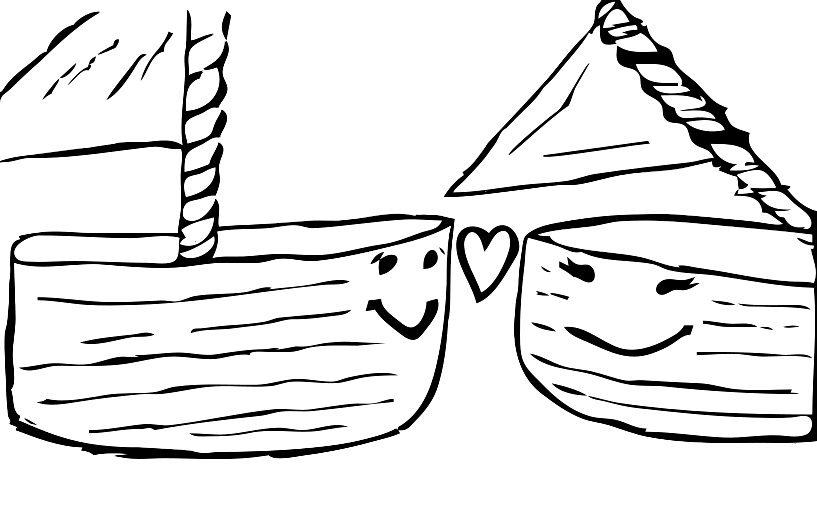
\includegraphics[width=5cm]{../bilder/fardigabilder/Batlat.png} 
	\end{center}
\end{intersong}